\section*{Question 1}
\emph{Plot the Probability Density Function (PDF) of the streamwise velocity from both datasets and calculate its first four moments. Using the moment information, comment on type of distribution exhibited by the two sets of data.}

\begin{figure}[!ht]
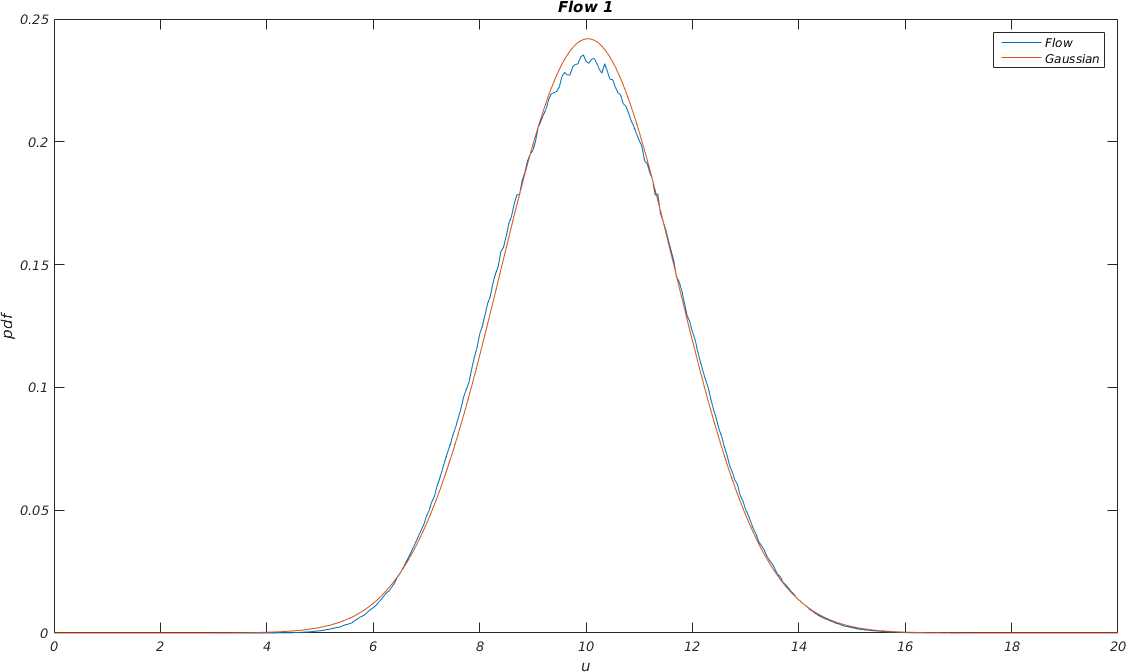
\includegraphics[scale=0.5]{./TEXT/pdf1.png}\label{pdf1}
\caption{The Probability Density function for \emph{flow 1}}
\end{figure}

Figures \ref{pdf1} and \ref{pdf2} show the probability density functions for the two flows with bin sizes of $0.05 m/s$. From these figures it can be seen that they respect a \emph{Gaussian} or \emph{Normal} distribution. Table \ref{tbl1} shows that the statistical data for the two cases is not different between the two cases.

\begin{table}[ht]
\caption{Comparison of the first four moments for the two flows.}
\label{tbl1}
\centering
\begin{tabular}{l|c|c}
& Flow 1 & Flow 2 \\
\hline
1\su{st} Moment: Mean & $10.04$ & $10.04$ \\
\hline
2\su{nd} Moment:Variance & $2.72$ & $2.72$ \\
\hline
3\su{rd} Moment:Skewness & $0.05$ & $0.05$\\
\hline
4\su{th} Moment:Kurtosis & $2.78$ & $2.78$ \\
\hline
\end{tabular}
\end{table}

\begin{figure}[!ht]
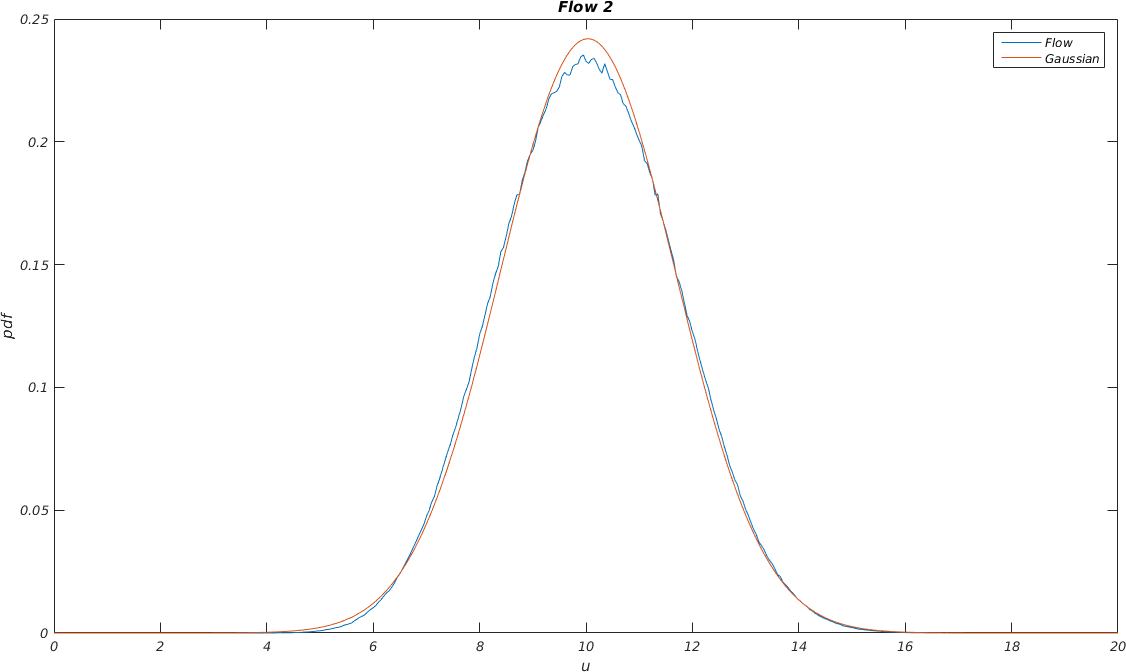
\includegraphics[scale=0.5]{./TEXT/pdf2.png}\label{pdf2}
\caption{The Probability Density function for \emph{flow 2}}
\end{figure}
